%-------------------------------------------------------------------------------
% seq64_playlist
%-------------------------------------------------------------------------------
%
% \file        seq64_playlist.tex
% \library     Documents
% \author      Chris Ahlstrom
% \date        2018-09-15
% \update      2018-09-16
% \version     $Revision$
% \license     $XPC_GPL_LICENSE$
%
%     Provides a discussion of the MIDI GUI playlist that Sequencer64
%     supports.
%
%-------------------------------------------------------------------------------

\section{Sequencer64 Play-Lists}
\label{sec:playlist}

   We have added a play-list feature to \textsl{Sequencer64}.
   This section consolidates the description of the play-list support.

   A play-list is a variation on the "rc" file, conventionally ending with the
   extension \texttt{.playlist}.  It contains a number of "playlist" sections,
   each with a human-readable title, selectable via a MIDI control number.
   Each playlist section contains a list of songs, each selectable via a MIDI
   control number or by moving to the next or previous song in the list.

   Movement between the playlists and the songs is accomplished via 
   MIDI control; see
   \sectionref{subsec:seq64_rc_file_midi_control}.
   It can also be done manually via the four arrow keys on the computer
   keyboard.
   Using MIDI control makes it possible to use the \texttt{seq64cli}
   headless version of \textsl{Sequencer64} in a live setting.

   The playlist can be specified on the command-line, or in
   the "rc" file (see \sectionref{subsec:seq64_rc_file_playlist}).
   If it is specified on the command line, that playlist setup will
   be written to the "rc" file.

   The play-list format is defined in the following section.
   Later sections describe the various user-interfaces.

\subsection{Sequencer64 Play-Lists / Format}
\label{subsec:playlist_setup}

   The play-list file, by convention, has a file-name of the form
   \texttt{sample.playlist}.
   The play-list file starts with a hardwired top banner that the user can edit
   with a text editor.  It can also have an optional comments section, much
   like the "rc" and "usr" files.  It is \textsl{not} overwritten
   when \textsl{Sequencer64} exits.

   \begin{verbatim}
   [comments]

   Comments added to this section are preserved.  Lines starting with
   a '#' or '[', or that are blank, are ignored.  Start lines that must
   be blank with a space.
   \end{verbatim}

   A blank line (not even a space) ends the comment section.

   Following the comments section are one or more \texttt{[playlist]} sections.
   Here is the layout of a sample playlist section.

   \begin{verbatim}
   [playlist]

   # Playlist number, arbitrary but unique. 0 to 127 recommended
   # for use with MIDI playlist control.
   126

   # Display name of this play list.
   "Music for Serious Dogs"

   # Storage directory for the song-files in this play list.
   contrib/midi/

   # Provides the MIDI song-control number, and also the
   # base file-name (tune.midi) of each song in this playlist.
   # The playlist directory is used, unless the file-name contains its
   # own path.
   70 allofarow.mid
   71 CountryStrum.midi
   72 contrib/wrk/longhair.wrk
   \end{verbatim}

   \index{playlist!tag}
   A play-list file can have more than one \texttt{[playlist]} section.  This
   allows for partitioning songs into various groups that can be easily
   selected (e.g. based on the mood of the musician or the audience).

   \index{playlist!number}
   After the \texttt{[playlist]} tag comes the play-list number.
   This number can be any non-negative value.
   However, in order to use MIDI control to select the playlist, this number
   should be limited to the range 0 to 127.
   If there is more than one \texttt{[playlist]} section, they are ordered by
   this number, regardless of where they sit in the play-list file.

   \index{playlist!title}
   Next comes a human-readable name for the playlist, which is meant to be
   displayed in the user-interface.  If surrounded by quotes, the quotes are
   removed before usage.

   \index{playlist!song-storage directory}
   Next is the song-storage directory.
   This directory is the default location in which to find the songs.
   It can be an absolute directory or a relative directory.
   However, be wary of using relative directories, since they depend on where
   \textsl{Sequencer64} is run.
   Also, if a song's file-name  has its own directory component, that overrides
   the default song-storage directory.

   Lastly, there is a list of MIDI song file-names, preceded by their numbers.
   As with the playlist numbers, it is recommended to keep them between 0 and
   127, for usage with MIDI control.  And the songs are ordered by this number,
   rather than by their position in the list.

\subsection{Sequencer64 Play-Lists / "rc" File}
\label{subsec:playlist_rc_file}

   The most consistent way to specify a play-list is to add an entry like the
   following to the "rc" file:

   \begin{verbatim}
   [playlist]
   # Provides a configured play-list and a flag to activate it.
   0     # playlist_active, 1 = active, 0 = do not use it
   # Provides the name of a play-list.  If there is none, use '""'.
   # Or set the flag above to 0.
   /home/ahlstrom/.config/sequencer64/sample.playlist
   \end{verbatim}

   This setup allows a play-list file to be specified and activated.
   If the name of the play-list file does \textsl{not} contain a directory,
   then the play-list file is search for in the user's \textsl{Sequencer64}
   configuration directory.

   If the play-list file-name is empty (i.e. set to \texttt{""}, then there is
   no play-list active.

\subsection{Sequencer64 Play-Lists / Command Line Invocation}
\label{subsec:playlist_cmd_line}

   The command-line options to specify (and activate) the play-list feature
   are:

   \begin{verbatim}
      -X playlist_file
      --playlist playlist_file
   \end{verbatim}

   The play-list file is either a base-name (e.g. \texttt{sample.playlist})
   or a name that includes the full path to the play-list file
   (e.g. \texttt{data/sample.playlist}).
   If no path is specified, the directory is the currently set
   \textsl{Sequencer64} configuration-file directory.

   Please note that any play-list file specified on the command line
   will be written into the "rc" file's \texttt{[playlist]} section when
   \textsl{Sequencer64} exits.

\subsection{Sequencer64 Play-Lists / Verification}
\label{subsec:playlist_verify}

   Currently, when \textsl{Sequencer64} loads a play-list file, every
   song in the file is verified by loading it.  If any load fails, then
   the playlist will fail to load.

   We may add an option to avoid that check, though it goes fast on
   modern hardware.

\subsection{Sequencer64 Play-Lists / User Interfaces}
\label{subsec:playlist_uis}

\subsubsection{Sequencer64 Play-Lists / User Interfaces / Gtkmm-2.4}
\label{subsubsec:playlist_ui_gtk}

   The Gtkmm-2.4 user-interface is currently the normal user-interface.
   However, it will ultimately be overtaken by the Qt 5 user-interface.
   So, for Gtkmm-2.4, \textsl{Sequencer64} merely allows the selection of the
   play-list and its songs via the four arrow keys, and it simply displays the
   current play-list name and the current song in the main window.

   The \texttt{Up} and \texttt{Down} arrows move forward or backward through
   the list of play-lists, and the
   The \texttt{Right} and \texttt{Left} arrows move forward or backward through
   the list of songs for the currently-selected play-list.

\subsubsection{Sequencer64 Play-Lists / User Interfaces / Qt 5}
\label{subsubsec:playlist_ui_qt}

   The Qt 5 user-interface will eventually become the standard.
   And it will (soon) support the full display, selection, and editing of the
   play-lists and the song-list for each play-list.
   The current playlist tab supports viewing the play-lists and songs, but not
   yet editing them.

\begin{figure}[H]
   \centering 
   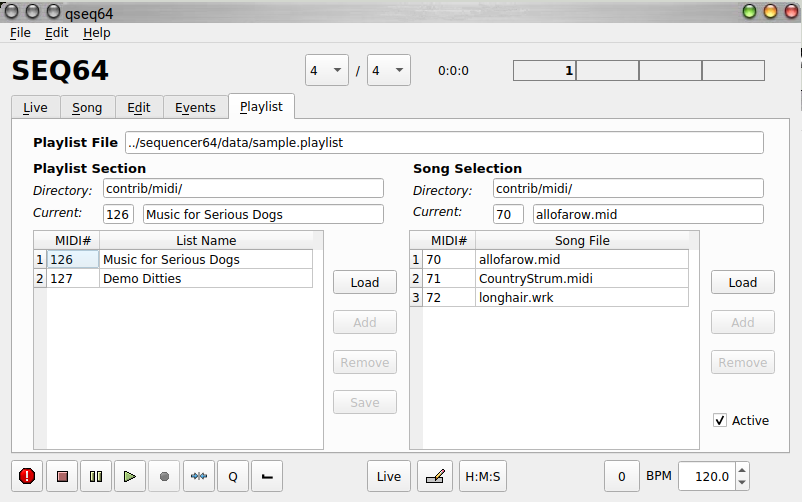
\includegraphics[scale=0.75]{qt/qt5_playlist_tab.png}
   \caption*{Qt 5 Playlist Tab}
\end{figure}

   Actually, the playlist currently has to be loaded from the command line or
   from the \textbf{File} menu.

%-------------------------------------------------------------------------------
% vim: ts=3 sw=3 et ft=tex
%-------------------------------------------------------------------------------
